\documentclass[a4paper,11pt,openany]{report}
\usepackage{subfigure}
\usepackage{graphicx}
\usepackage [utf8]{inputenc}
\usepackage{url}
\usepackage{float}
\usepackage{enumerate}
\usepackage{subfig}
\usepackage{pifont}
\usepackage{tabularx}
\usepackage{listings}
\usepackage[table]{xcolor}

\title{Crosscompilation of the open source web browser engine WebKitGTK+ for the ARMv7 processors family}
\author{Antonio Arias Losada}
\date{1st October 2012}
\begin{document}
\maketitle
\tableofcontents
\listoffigures
\listoftables

\chapter{Introduction}
This document resumes the work carried out during the Free Software Master\cite{master} Practicum developed by Antonio Arias, in 2012. This Master is taught by Igalia and Rey Juan Carlos University, and the Practicum is the final work done in this Master studies as a real environment exercise related with open source technologies.

In this particular case the Practicum work involves the crosscompilation of the WebKitGTK+\cite{webkitgtk+} web browser engine for the ARMv7 processors family, which is one of the more extended processors families in the embedded developments. This will virtually enable a huge number of embbeded devices to run one of the more powerful web browser engines, allowing to create web applications based on the latest HTML technologies and been able to be used almost everywhere.

In this Practicum project, to achieve its goal, they were used some technologies related with embedded environments, as the ARMv7 processor family selected target, the Yocto\cite{yocto} and OpenEmbedded\cite{openembedded} crosscompilation toolchains used for the compilation tasks, and the QEMU\cite{qemu} processor emulation software, to test the resulting compiled images. All of these, less ARMv7, which is a proprietary hardware architecture, are free software.

Following these enumerated technologies are introduced.

\section{Yocto project}
The Yocto project is an open source collaboration project that provides templates, tools and methods to help you creating custom Linux-based systems for embedded products regardless of the hardware architecture. It's not an embedded Linux distribution, it creates a custom one for you.

Traditionally the Linux distribution porting to different architectures, specifically to embedded systems, used to be a hard task with a lot of custom work related with the low level hardware layer adaptation, known as hardware abstraction layer (HAL).

In order to try to manage this tasks in a more simple way, some toolchains were created. The historic evolution of the Yocto project, that represents an example of the creation of this kind of toolchains, was as follows:

\begin{itemize}
\item In the year 2001, Sharp introduces the SL-5000, a PDA that runs a Linux based operating system.
\item In the year 2002, Chris Larson, realized that the original Sharp ROM is quite limited and he decided to start working on a new build system, OpenZaurus\cite{openzaurus}, to create custom ROM image for this device.
\item During the years 2002 and 2003, OpenZaurus project grew and started supporting a large number of packages and targets, based on Buildroot\cite{buildroot} tools.
\item In January 2003, some limitations of Buildroot are clear, and BitBake\cite{bitbake} creation was proposed as a solution.
\item In February 2003, Holger Schurig, started the OpenEmbedded development, based on BitBake.
\item In May 2003, Chris Larson, added the mayor functionality from OpenZaurus to the OpenEmbedded project, and started the convertions of the other packages.
\item In December 2003, Michael Lauer, released the version 3.3.5 of the OpenZaurus project, and abandoned the OpenZaurus build system, and converted hundreds of packages to OpenEmbedded.
\item In December 2004, the OpenEmbedded project splitted its development into the BitBake build system, as a generic task executor, and the OpenEmbedded metadata for BitBake.
\item OpenEmbedded was merged with some contributions from projects like Faliar Linux and OpenSIMpad, getting a common codebase, from which any of the original projects could be built.
\item Other distros started adapting OE: Unslug, OpenSimpad, GPE Phone Edition, {\AA}ngstr\"om, OpenMoko... 
\item 2006-2008 Linux Start-Up OpenedHand developed a distribution called Poky Linux\cite{poky} (and the Clutter library).
\item 2008 Intel buys OpenedHand; focus for Poky is now on Atom based devices
\item 2010 Linux foundation starts Yocto Project: x86, ARM, MIPS, and Power Architecture
\item 2011 Work on common code base with OpenEmbedded: OpenEmbedded-Core 
\end{itemize}

The Yocto project is licensed under a mix of licenses of GPLv2 and MIT.

\section{QEMU}
QEMU (Quick Emulator) is an open source software capable of emulate or virtualize a bunch different processor families, including most of the more common architectures in embedded systems, like PowerPC, MIPS, or ARM. It also can emulate common x86 PC architectures.

As an emulator it uses dynamic binary translation, which consists in the translation of the instruction sets, from the ones of the emulated architecture into code undestandable by the host device. This emulation technique can achieve a reasonable execution speed, getting an easy scalable solution to emulate new architectures.

It can work in two different modes, emulation or virtualization. When it is used as an emulator, it can run operating systems or any other software built to an architecture different from the host machine one.

When it is used to virtualize a different machine, it can achieve a performance close to the native one, executing the guest code directly on the host processor. The virtualization is done with the support of the Xen hypervisor or using the KVM kernel module in Linux. The targets that can be virtualized are x86, PowerPC and S390 processors.

QEMU is released under GPL v2 license.

\section{ARMv7}
The ARM (Advanced RISC Machine)\cite{arm} is a processor architecture of 32 bits. It is one of the more spread processors architectures in embedded systems, due to its simplicity and low power consumption. Its growth is supported by the licensing policy, which makes possible that a large number of different manufacturers can implement its solution based on this architecture, getting a huge number of developers specialized in this architecture.

The ARMv7 processor core defines the base instruction set more used in the nowadays ARM processor implementations.

With the ARMv7 family also appeared some architecture extensions like Thumb, which creates a 16 bits sub instruction set to reduce the code size of the more common software parts, or Jazelle, responsible of Java bytecode native execution.

\section{WebKit}
WebKit\cite{webkit} is an open source web browser engine, used as the basis for powerful web browsers like Epiphany, Safari or Google Chrome.

Its development was started in 1998, as part of the KDE project, under the name of KHTML with the JavaScript engine KJS. Based on these projects, Apple announced in 2002 its forks called WebCore and JavaScriptCore, and in January 2003 Apple relased both cores as open source, under the name of WebKit. They released in 2003 their Safari web browser for the first time based in this new open source web browser engine.

On the $8^{th}$ of april of 2010 was announced a new version of WebKit, that was redesigned from the scratch to get a multi process web engine, where each web application is executed as an independant process. This new version produced an incompatible API, and this caused that this new version should have a different name to try to avoid confusions, so it was called WebKit2.

WebKitGTK+, the target of this Practicum work, is the porting of the WebKit web engine to run under the GTK+\cite{gtk+} platform, which is a multi-platform for creating graphical user interfaces, based on the initial development of GIMP\cite{gimp} project, and now as part of the GNOME\cite{gnome} project.

The WebKit project is licensed under the LGPL and BSD licenses.

\chapter{Description of the practicum}

\section{About the author}
The author of this Master Thesis is Antonio Arias Losada, student of the Free Software Master, in the 2012 edition.
Antonio is Telecommunication Engineer by the Vigo University in 2006. He has experience in programming in several general purpose languages, mainly in Java and ANSI C, working from 2005 to ending of 2006 developing telephony applications. From 2007 to 2009 he worked as Embedded Engineer in the automotive sector. From 2009 until now he has been working in the design, development and management of embedded devices and systems in the medical sector.

\section{About the tutor}
The tutor of this Master Thesis is V\'ictor Manuel J\'aquez Leal. He is a software engineer with solid experience in GNU/Linux mobile device development, focused on hardware accelerated multimedia and system applications (package management), and interested in kernel space development.

\section{The hosting enterprise}
The hosting enterprise of this Practicum project is Igalia\cite{igalia}. Igalia is a Free Software Engineering company, focused on selling services and knowledge.

It is a company based on 3 main values:

\begin{itemize}
\item Flat organizational structure 
\item Free software
\item Innovation and research
\end{itemize}

Igalia employes several core developers of the WebKitGTK+ port, with contributions including bugfixing, performance, accessibility, API design and many major features. It also provides various parts of the needed infrastructure for its day to day functioning, and is involved in the spread of WebKit among its clients and in the GNOME ecosystem, for example leading the transition of the Epiphany web browser to WebKit.

\section{Practicum description}
WebKit is one of the more complete and versatile web browser engines, with a high level of standard compatibility, used in some of the more important web browser applications, and huge number of embedded devices. This becomes WebKit in an very important piece of code in the nowadays world, where the web applications are becoming a key point in the software ecosystem.

This practicum was focused in the crosscompilation of the open source web browser engine WebKitGTK+ to be used in a ARMv7 based system, one of the more used processors families in the embedded devices availables in the market. 

\section{Practicum planning and work environment}
Usually this practicum work used to be done during the summer time, mainly in July and August. The author of the practicum has a full time job, which makes impossible to dedicate the needed time to the practicum work only on summer. Trying to solve this problem this work was started earlier. So it was planned in short working days of 3 hours each, from Monday to Friday, starting on 14th of May and ending on 30th of September. This way it should be spent about 300 hours on practicum work.

The work was planned to be done at home, having a weekly report by email from the author to the tutor, in order to keep him informed about the progress and problems. It was also planned periodic phone conferences for a deeper revision of the work.

The author kept a log file with all the information and steps he gathered during his work progress. This notes allow him to keep a track of his advances in the work, and a history view of the work.

The main goal of the practicum work was described to be able to run an emulated environment using QEMU, which makes possible to make all the work only with a personal computer, without any special extra needs.

Otherwise, it was stablished, as an extra objetive just the main goal was reached quite early, running the generated image in a real target like an evaluation board of a ARMv7 processor.

This practicum work involves the usage of the WebKit web browser engine, focused in its compilation, getting and managing its dependencies. But most of the work is centred on Yocto Project, learning its architecture, and how to use it.

\chapter{Work plan}

\section{Objectives}
The main objective of the Practicum is getting a crosscompiled Linux image, ready to run a WebKit based browser, for an ARMv7 architecture processor. This was planned to be got with some milestones:

\begin{itemize}
\item Compiling WebKit for x86 or amd64 architecture, getting a functional WebKit demo web browser.
\item Prepare Yocto environment.
\item Create a Yocto image and run it using QEMU.
\item Create a Yocto with WebKit, getting a functional WebKit demo web broser for ARMv7 architecture, and run it using QEMU.
\end{itemize}

As a guide to support the creation of the Yocto image with a WebKit browser in it, it was planned to use the meta-browser\cite{meta-browser} layer, and as an extra objective, it was planned getting a patch to be sent to this Yocto layer project.

\section{Motivation}
The HTML5 improvements, which increases the web development capabilities to build full applications becomes more important the web browser role.

This is also applicable for the development of embedded applications, using a web browser for the user interface of embedded devices.

One of the more powerful and flexible solutions to create a web browser is using WebKit, an open source web browser engine. That is the main motivation of this Practicum project, that tries to compile one of the best web browser solutions for one of the more extended embedded processor architetures.

\section{Methodology}
The work in this practicum project was planed to be done in consecutive iterations, getting step by step the main goal fo the project.

The first step is getting the WekKit environment compiled for a personal computer target, learning how to compile this web browser engine, with its web browser example, taking note of the needed dependencies. This should set the basis for the future crosscompilation.

When the first step is done, the next one consists in getting a Yocto environment ready. This task consist in getting the software environment install and ready to create Linux images for different architectures, and also in investigating the Yocto Project documentation, learning how the environment is used to create the images.

With the Yocto environment ready, the next task is creating an ARMv7 image, based on the default ones included in the Yocto Project. Once this image is created, it should be runnable using QEMU emulator.

Finally, it should be prepared an image with a WebKit environment compiled, satisfying all its dependencies, running this image using QEMU as in the previous step.

In order to facilitate the work, and to point its evolution towards the extra objective, the recipes are based on meta-browser Yocto layer.

\section{Workplan}
Just after the main goals of the Practicum work were described, the planning calendar was stablished, trying to distribute the work in the available time until the ending of the Practicum period, and having in mind the stimated time that were going to be dedicated.
This process defined the following calendar, based on milestones and periodic meetings to keep track of the work progress:
\\
\begin{table}
\begin{tabularx}{\textwidth}{|c|c|X|X|}
\hline 
Week & Month & Task & Meeting \\ 
\hline 
w20 & May &  &  \\ 
\hline 
w21 &  & 1. Desktop WebKit compilation & Meeting (24/05/2012) \\ 
\hline 
w22 & Jun &  &  \\ 
\hline 
w23 &  &  &  \\ 
\hline 
w24 &  &  &  \\ 
\hline 
w25 &  &  &  \\ 
\hline 
w26 &  &  &  \\ 
\hline 
w27 & Jul & 2. Yocto environment & Meeting (05/07/2012) \\ 
\hline 
w28 &  &  &  \\ 
\hline 
w29 &  &  &  \\ 
\hline 
w30 &  &  &  \\ 
\hline 
w31 & Aug & 3. Run generated image in QEMU & Meeting (02/08/2012) \\ 
\hline 
w32 &  &  &  \\ 
\hline 
w33 &  &  &  \\ 
\hline 
w34 &  &  &  \\ 
\hline 
w35 & Sep & 4. WebKit compilation in Yocto and running it in QEMU & Meeting (30/08/2012) \\ 
\hline 
w36 &  &  &  \\ 
\hline 
w37 &  &  &  \\ 
\hline 
w38 &  & 5. Report &  \\ 
\hline 
w39 &  & 5. Report & Meeting (27/09/2012) \\ 
\hline 
\end{tabularx}
\caption{Workplan schedule}
\end{table}

\chapter{Results}
The work was started as it was expected and planned. In the following sections are described the detailed results of each planned task.

\section{Task 1: Desktop WebKit compilation}
The \textbf{task 1} was done with a delay of a week over the planning. It consisted of getting the WebKit code, reading the building WebKitGTK+\cite{build webkitgtk+} documentation, and compiling it.
For the first time it was tried to download the WebKit code using its official SVN repository, but it was so hard, because there is a lot of code to download and the repository checkout failed all the times it was tried. Then it was done cloning the git repository of WebKit\cite{git webkit}, which took about 3 hours to be done, but it worked on the first time.
While the repository was been cloned, the documentation reading was done, and this helps saving some time.

The compilation process was done using a chroot\cite{chroot} environment, been helped with the debootstrap\cite{debootstrap} tool, configuring a sandbox with a fully operational Debian testing operating system, avoiding dirting the base system with the tests.
After adding all the dependencies, cited on the building WebKitGTK documentation, to the sandboxed Debian OS just using apt-get command, WebKitGTK+ could be compiled. It took about an hour to be done. Once it had finished it gives this message:

{
\footnotesize
\begin{lstlisting}
===========================================================
 WebKit is now built (1h:04m:54s).
 To run GtkLauncher with this newly-built code, use the
 "Tools/Scripts/run-launcher" script.
===========================================================
\end{lstlisting}
}

But after running the \verb#run-launcher# script fails with the message:

{
\footnotesize
\begin{lstlisting}
$ ./Tools/Scripts/run-launcher
Unsupported platform, can't determine built library locations.
Try `build-webkit --help` for more information.
\end{lstlisting}
}

After reading some times the documentation, and looking for some examples, the problem was solved just adding the parameter \verb#--gtk# when running the \verb#run-launcher# script, in the way:

{
\footnotesize
\begin{lstlisting}
$ ./Tools/Scripts/run-launcher --gtk
\end{lstlisting}
}

This runs a simple web browser example based on the compiled WebKit engine, that could be considered as the task 1 goal achieved in the week 22, one later than planned.

\begin{figure}[hbtp]
\centering
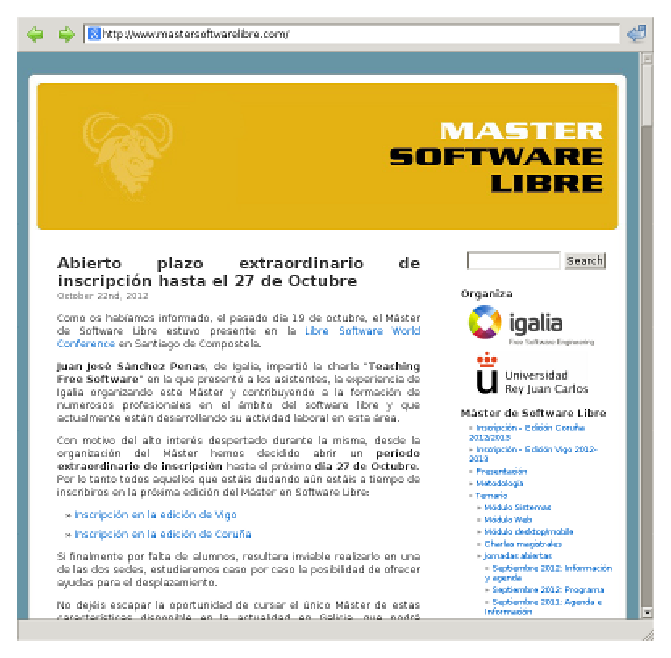
\includegraphics[scale=1]{webkit_x86.eps}
\caption{WebKitGTK+ x86}
\end{figure}

\section{Task 2: Yocto environment}
The \textbf{task 2} was started on time, in the week 22, been run on pararell with the task 1 ending. It was formed by the Yocto Project documentation reading, and the environment preparation.
The environment preparation was made following the Yocto project quick start guide\cite{yocto quick start}. This guide states the Ubuntu, Fedora, openSUSE and CentOS distributions, in the previous version to the last one, as the tested ones. But for the first test it was tried to deploy it using the Debian chroot environment previously used in the task 1, but it failed. After some trials to solve the problems, a new chroot environoment based on a Ubuntu 11.10 distribution was created, and the Yocto toolchain was tested successfully in this new sandbox. The task was ended in the week 24, before than expected in the initial planning.

\section{Task 3: Run generated image in QEMU}
The \textbf{task 3} was started in the week 24, about the creation of an image and running it using QEMU. It was selected the \verb#core-image-sato# Yocto demo image to get this done. Two test were done, one with a x86 target and the other with an ARM target. This was done in the week 25. While this compilations are done, some investigations about who creating custom recipes were done, just to advance in the next task work.

In the week 26 a problem about the work done until that moment was discovered. The problem was about the specific ARM target that was been used. The ARM target the image was compiled to was ARMv5, and not ARMv7 as it was defined in the Practicum objectives.

A solution was proposed by the tutor to configure the Yocto environment to compile for a ARMv7 target. This solution was changing the Yocto environment configuration in the file \verb#conf/machine/qemuarm.conf#, cambiando la línea \verb#require conf/machine/include/tune-arm926ejs.inc# por \verb#require conf/machine/include/arm/arch-armv7a.inc#.

This creates an environment capable of compiling for ARMv7 processors, but another problem related with the emulator appeared. When running the emulator with any image created this way, it results in a Kernel Panic error.

\section{Task 4: WebKit compilation in Yocto and running it in QEMU}
The \textbf{task 4} was started around the week 32, but most of the time since then was used to try to solve the Kernel Panic issue, but any of the efforts were productive, with the problem that any new compilation trial was too long. In paralell were made some recipes creations, but they were quite a black box job, due to the imposibility of a real testing.

This task was stopped in the week 39, because it was delaying too much the start of the task 5, about the creation of this report.

The work done during this task was quite incomplete, so the results of it were quite poor at this moment, and it was planned to be improved and finished after the creation of this document.

\begin{figure}[hbtp]
\centering
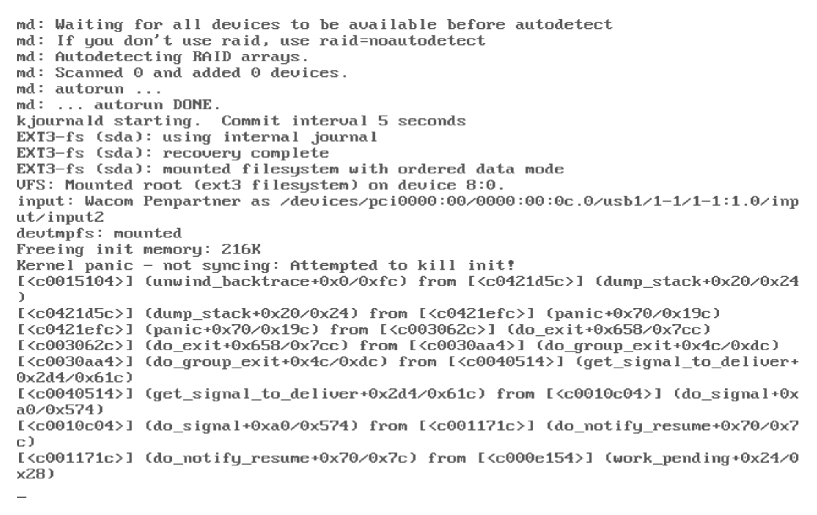
\includegraphics[scale=1]{kernel_panic.eps}
\caption{Kernel Panic}
\end{figure}

\chapter{Future work}
At the moment of writing this document, the identified future work in a very short term is finishing the Linux image creation, containing a WebKitGTK+ web browser for ARMv7 processor target, running it in the QEMU emulator, because despite it was the Practicum work main objective it could not be achived on time.

Once the planned work is completed the following work would be testing this compiled image in a real embedded device target, verifying its behaviour in a real environment. This would be very useful to test if all the requirements are satisfied to run the resulting image in a real environment, enabling to test its performance too.

As in the initial planning, the next goal would be creating a patch to be sent to the meta-browser Yocto layer project. This task would become the made work in reusable by any other person interested in running a WebKit web browser in a ARMv7 processor.

As a final objective, that is planned to be done in a future work, would be creating a image for ARMv7 using the OSTree\cite{ostree} tool. This tool enables to manage the creation of one or multiple file system images, creating a easy method of managing the new features integration, while keeping a fully functional system. It could be easyly described as a ``Git-like tool for storing entire snapshots of an operating system''.

\chapter{Personal evaluation}
The work done in this Practicum project was very helpful for the author for his learning about the usage of the crosscompiling tools, and the porting of some pieces of code to embedded platforms.

It was very intersting and useful learning how to use the tools chroot and debootstrap, which facilitate the testing process with different libraries and system configurations, avoiding using in several times virtual machines, that makes the host computer to go slower with a high memory consumption.

His expertise about the embedded systems was limited in this field due the fact that he had always used dedicated tools to build custom firmware pieces of code. This was a good start point to learn how to customize a Linux distribution for embedded systems.

The initial planning seemed acute and realistic to be done in 300 hours of work time. But this changed during the course of the Practicum, because the 300 hours were planned to be done in small fragments of 3 hours a day, and some times this time got shorter but recovered during the weekend. This time fragmentation reduced the available time usefulness.

This fact got worse due to the very long testing cycles of the different trials. Each WebKit compilation took about X hours, and each Yocto compilation took about X hours, so each full test was too long, so the failures were too expensive, and they become the initial timing in optimistic in some way.

To try to minimize the impact of this long testing cycles, they were make most of the time on night, other times during the working day, using remote connection to the computer from the office, and the rest of the thest were done taking advance of the reading documentation time.

The first long tests were a bit optimistic, and they were not so productive due to the lack of notes about was the testing is trying to do, and its long duration combined with the short daily quantum time for the Practicum work, made that in this first test were lost the focus of some tested details.

This was minimized with some fast notes took just when the test was started, just to keep the context of the test while it is done.

The global personal evaluation from the point of view of the author is positive. Perhaps at the moment of writing this report about the work done during the Master Practicum the main goal of it was not reached, but the right way was stablished, and a lot of technical and planning issues were leart.

After this report was finished, the work to get a fully functional recipe to compile WebKit using Yocto project for the ARMv7 processors family is going to continue, having in mind to complete it.

\begin{thebibliography}{ZZ}

\bibitem{master}
Free Software Master\\
\url{http://www.mastersoftwarelibre.com/}

\bibitem{igalia}
Igalia\\
\url{http://www.igalia.com/}

\bibitem{yocto}
Yocto Project\\
\url{http://www.yoctoproject.org/}

\bibitem{yocto quick start}
Yocto Project Quick Start Guide\\
\url{http://www.yoctoproject.org/docs/current/yocto-project-qs/yocto-project-qs.html}

\bibitem{qemu}
QEMU\\
\url{http://www.qemu.org/}

\bibitem{arm}
ARM\\
\url{http://www.arm.com/}

\bibitem{webkit}
WebKit\\
\url{http://www.webkit.org/}

\bibitem{build webkitgtk+}
Building WebKitGTK+\\
\url{http://trac.webkit.org/wiki/BuildingGtk/}

\bibitem{git webkit}
Tips and Tricks for using Git with WebKit\\
\url{http://trac.webkit.org/wiki/UsingGitWithWebKit/}

\bibitem{webkitgtk+}
WebKitGTK+\\
\url{http://webkitgtk.org/}

\bibitem{gtk+}
GTK+\\
\url{http://www.gtk.org/}

\bibitem{gimp}
GIMP\\
\url{http://www.gimp.org/}

\bibitem{gnome}
GNOME\\
\url{http://www.gnome.org/}

\bibitem{meta-browser}
meta-browser: OpenEmbedded/Yocto BSP layer for Web Browsers\\
\url{https://github.com/OSSystems/meta-browser}

\bibitem{openzaurus}
OpenZaurus\\
\url{http://www.openzaurus.org/wordpress/}

\bibitem{buildroot}
BuildRoot\\
\url{http://buildroot.uclibc.org/}

\bibitem{bitbake}
BitBake\\
\url{http://developer.berlios.de/projects/bitbake/}

\bibitem{poky}
Poky Linux\\
\url{http://www.pokylinux.org/}

\bibitem{openembedded}
OpenEmbedded\\
\url{http://www.openembedded.org/wiki/Main_Page}

\bibitem{chroot}
chroot\\
\url{http://www.kernel.org/doc/man-pages/online/pages/man2/chroot.2.html}

\bibitem{debootstrap}
debootstrap\\
\url{http://wiki.debian.org/Debootstrap/}

\bibitem{ostree}
OSTree\\
\url{https://live.gnome.org/OSTree/}

\end{thebibliography}

\end{document}
